%%****************************************************************************
%** Copyright 2002, 2003 by Lukas Ruf, <ruf@topsy.net>
%** Information is provided under the terms of the
%** GNU Free Documentation License <http://www.gnu.org/copyleft/fdl.html>
%** Fairness: Cite the source of information, visit <http://www.topsy.net>
%****************************************************************************
%** Last Modification: 2005-07-11 1600
%** 2005-07-11	Bernhard Tellenbach
%**							Switched default document class to: book
%**							Added \include{appendix.tex}
%****************************************************************************

%\documentclass[10pt,final,a4paper,twoside]{book}
%\documentclass[10pt,draft,a4paper,oneside]{report}
\documentclass[headings=optiontohead,10pt,final,a4paper,oneside]{scrreprt}
%\documentclass[10pt,draft,a4paper,oneside]{article}

%**Latex Master Document*********

%** preamble.tex: here all the document-wide settings
%                 are defined
\RequirePackage{times}

%\usepackage[english]{babel}
%-% \usepackage[german]{babel}
\usepackage[ngerman]{babel}

\usepackage[utf8]{inputenc}
\usepackage[T1]{fontenc}
\usepackage{textcomp}
\usepackage{type1cm}
\usepackage[table,xcdraw]{xcolor}
\usepackage{a4}

\usepackage{graphicx}
\graphicspath{{Figures/},{Pictures/}}
\usepackage{subfigure}

\usepackage{fancyhdr}
\usepackage{fancybox}
\usepackage{hyperref}

\usepackage{float}
\usepackage{longtable}
\usepackage{paralist}
\usepackage{url}
\usepackage{lscape}
\usepackage{moreverb}

\usepackage{makecell}
\usepackage{multirow}

\usepackage{tabularx}
\usepackage{xltabular}

\usepackage{nomencl}
  \let\abbrev\nomenclature
  \renewcommand{\nomname}{List of Abbrevations}
  \setlength{\nomlabelwidth}{.25\hsize}
  \renewcommand{\nomlabel}[1]{#1 \dotfill}
  \setlength{\nomitemsep}{-\parsep}
  %For old nomencl package, uncomment this:
  \makeglossary 
  %For new nomencl package, uncomment this:
  %\makenomenclature

\usepackage[normalem]{ulem}
  \newcommand{\markup}[1]{\uline{#1}}
  
   
\usepackage{ae,aecompl}


\usepackage[first,bottomafter,light]{draftcopy}
\draftcopyName{Draft v0.1}{120}

\addtolength{\textwidth}{2cm}
\addtolength{\textheight}{2cm}
\addtolength{\oddsidemargin}{-1.0cm}
\addtolength{\evensidemargin}{-1.0cm}
\addtolength{\topmargin}{-1.5cm}

%% No Serifs: Put comment markers in front of the next three lines otherwise
\renewcommand{\ttdefault}{cmtt}
\renewcommand{\rmdefault}{phv}  % Helvetica for roman type as well as sf
\renewcommand{\ttdefault}{pcr}  % use Courier for fixed pitch, if needed

\newcommand{\?}{\discretionary{/}{}{/}}
\newcommand{\liter}[0]{/home/ruf/Lib/Bibl/}
\newcommand{\fref}[1]{\mbox{Figure~\ref{#1}}}

\pagestyle{fancy}
%%-lpr Note: 'chapters' are defined for 'book's only
%%-lpr       in articles, we make use of sections only
\renewcommand{\chaptermark}[1]{\markboth{#1}{}}
\renewcommand{\sectionmark}[1]{\markright{\thesection\ #1}}
\fancyhf{}

%\fancyhead[LE,RO]{\bfseries\thepage}
%\fancyhead[LO]{\bfseries\rightmark}
%\fancyhead[RE]{\bfseries\leftmark}
\fancyhead[R]{\leftmark}
\fancyhead[L]{\rightmark}
\fancyfoot[R]{\thepage}
\fancyfoot[C]{ZHAW SoE}
\fancyfoot[L]{Bachelor Thesis (Informatik)}

\renewcommand{\headrulewidth}{0.5pt}
\renewcommand{\footrulewidth}{0.5pt}
\addtolength{\headheight}{0.5pt}
\fancypagestyle{plain}{%
   \fancyhf{}
   \fancyfoot[C]{\bfseries \thepage}
   \fancyhead{}%get rid of headers on plain pages
   \renewcommand{\headrulewidth}{0pt} % an the line
}
\newcommand{\clearemptydoublepage}{\newpage{\pagestyle{empty}\cleardoublepage}}

\setlength{\parindent}{0in}



\hyphenation{Strea-men}
\hyphenation{Apps}
\hyphenation{Threat}
\hyphenation{Init}

\newcommand{\Appendix}[2][?]
{
  \refstepcounter{section}
  \addcontentsline{toc}{appendix}
  {
    \protect\numberline{\appendixname~\thesection} %1
  }
  {
    \flushright\large\bfseries\appendixname\ \thesection\par
    \nohypens\centering#1\par
  }
  \vspace{\baselineskip}
}

\let\margin\marginpar
\newcommand\myMargin[1]{\margin{\raggedright\scriptsize #1}}
\renewcommand{\marginpar}[1]{\myMargin{#1}}

\newcommand\CHECK{\myMargin{CHECK}}
\newcommand\NEW{\myMargin{NEW}}

\usepackage[acronym,numberedsection=autolabel,section=section]{glossaries}

\makeglossaries

% \newacronym{<id>}{<short>}{<long>}

%\newglossaryentry{glos:mpegts}{
% name=MPEG Transport Stream,
% description={Von der Moving Picture Experts Group entwickeltes Transportstream-Protokoll für Video/Audio-Übertragung}
%}

\newacronym{ISP}{ISP}{Internet Service Provider}
\newacronym{OSS}{OSS}{Operations Support System}
\newacronym{NMS}{NMS}{Network Management System}
\newacronym{BSS}{BSS}{Business Support System}
\newacronym{CPE}{CPE}{customer premises equipment}
\newacronym{ADSL}{ADSL}{asymmetric digital subscriber line}
\newacronym{DSL}{DSL}{digital subscriber line}
\newacronym{VDSL}{VDSL}{very high-speed digital subscriber line}
\newacronym{PoP}{PoP}{point of presence}
\newacronym{B2B}{B2B}{business to business}
\newacronym{BGP}{BGP}{Border Gateway Protocol}
\newacronym{MPLS}{MPLS}{Multiprotocol Label Switching}
\newacronym{OSPF}{OSPF}{Open Shortest Path First}
\newacronym{FTTH}{FTTH}{Fiber To The Home}
\newacronym{FTTS}{FTTS}{Fiber To The Street}
\newacronym{OTO}{OTO}{Optical Telecommunication Outlet}
\newacronym{IRM}{IRM}{infrastructure resource modeling}

\newacronym{OMDF}{OMDF}{Optical Main Distribution Frame}
\newacronym{CLI}{CLI}{command line interface}

\newacronym{OHDF}{OHDF}{Optical Handover Distribution Frame}
\newacronym{IGP}{IGP}{Interior gateway protocol}

%% TODO: Definition Network Element

\newglossaryentry{glos:snmp}{
    name=Sinmple Network Management Protocol,
    description={}
}



\newglossaryentry{glos:isp}{
 name=MPEG Transport Stream,
 description={Von der Moving Picture Experts Group entwickeltes Transportstream-Protokoll für Video/Audio-Übertragung}
}


%\useshorthands*{"}
%\addto\extrasenglish{\languageshorthands{ngerman}}

\usepackage{csquotes}
\usepackage[
backend=biber,
bibstyle=ieee,
style=numeric,
sorting=none
]{biblatex}
\addbibresource{citations.bib}


\usepackage{pdfpages}
\usepackage{rotating}
\usepackage{pdflscape}

%% Adds another nesting level of numbering for sections
\setcounter{secnumdepth}{3}

\usepackage{helvet}
%\renewcommand*{\familydefault}{\sfdefault}

\usepackage{color,soul}

\usepackage[section,numbib,nottoc]{tocbibind}
\renewcommand{\listoffigures}{
    \tocsection
    \tocfile{\listfigurename}{lof}
}
\renewcommand{\listoftables}{
    \tocsection
    \tocfile{\listtablename}{lot}
}

%********************************

%** begin the document environment
\begin{document}

\frenchspacing
\sloppy

%** Titel.tex: Title page to be printed first

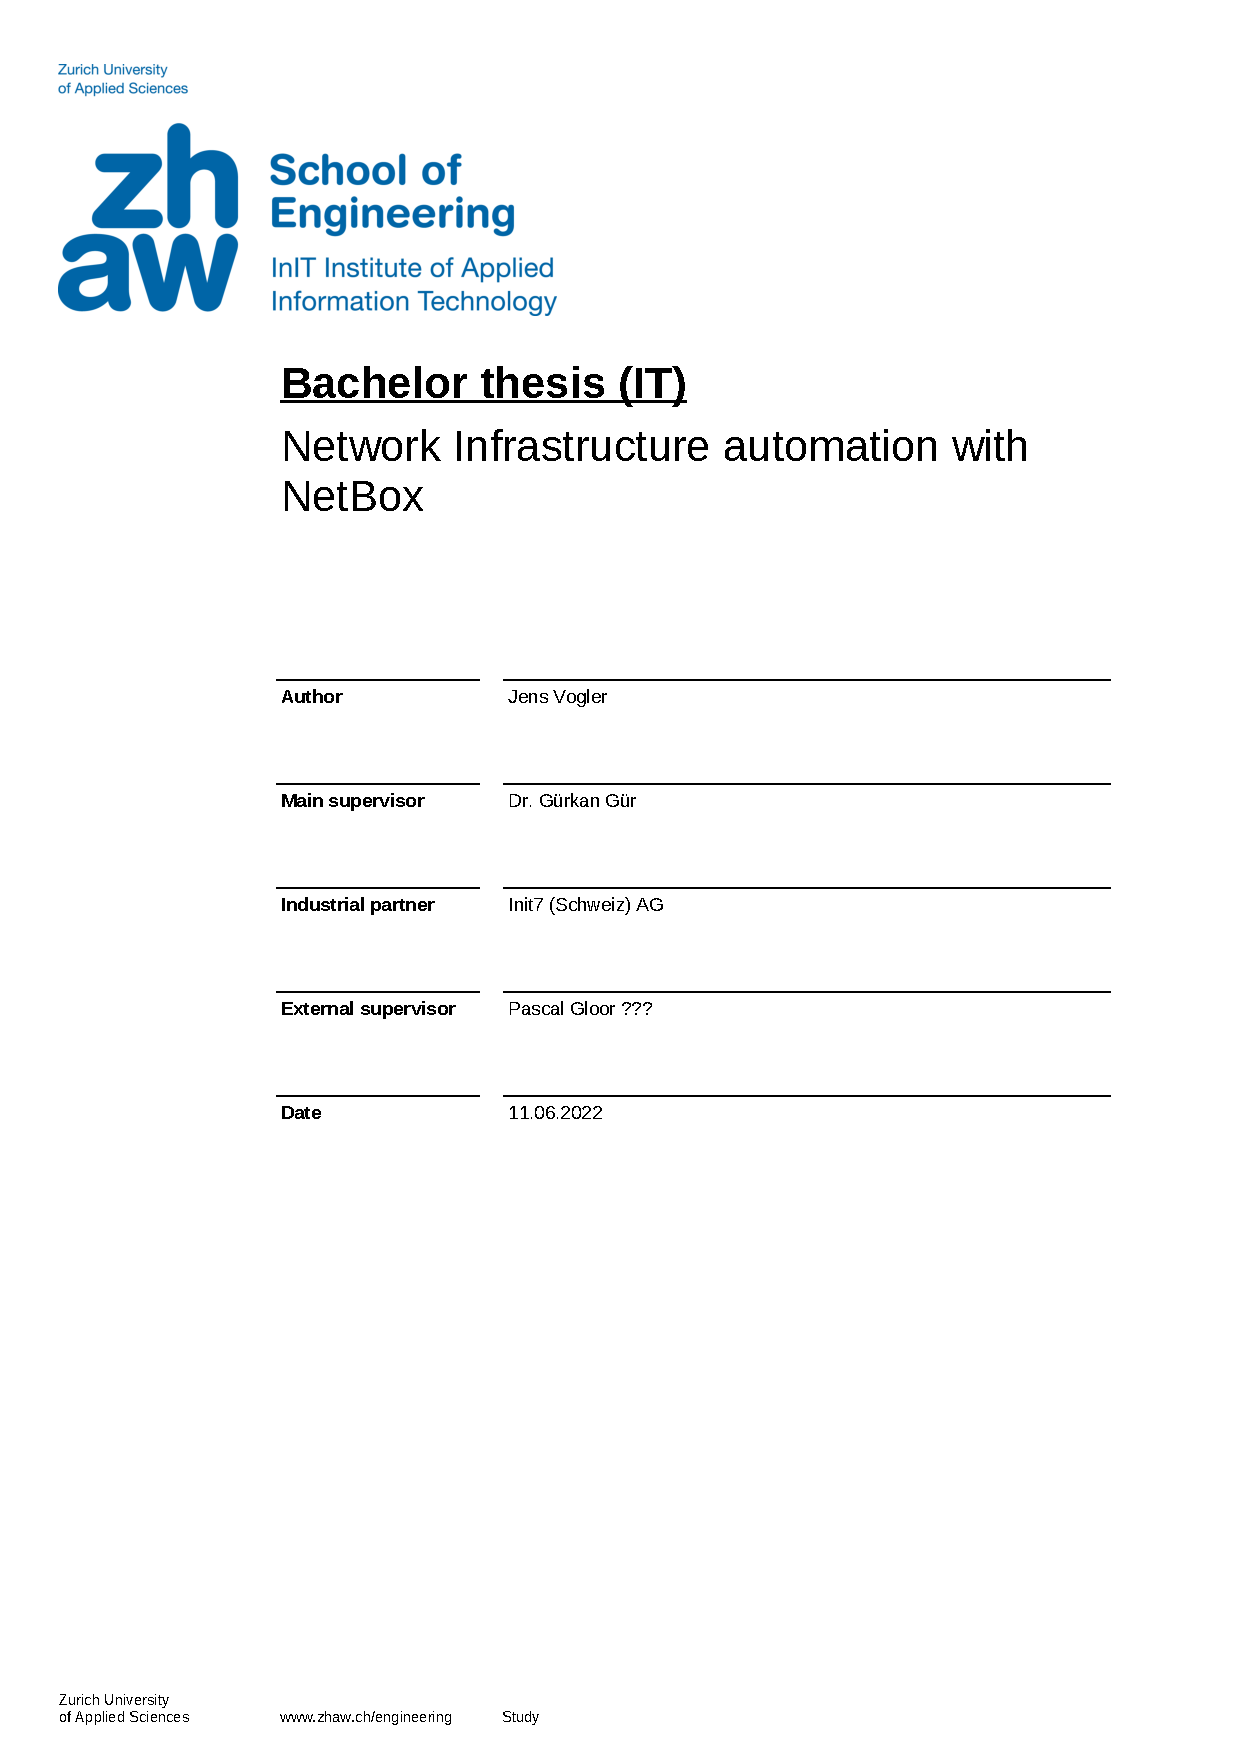
\includepdf[pages=-]{../Attachments/SoE-INIT_Bachelor-Titelblatt-Vorlage_en.pdf}
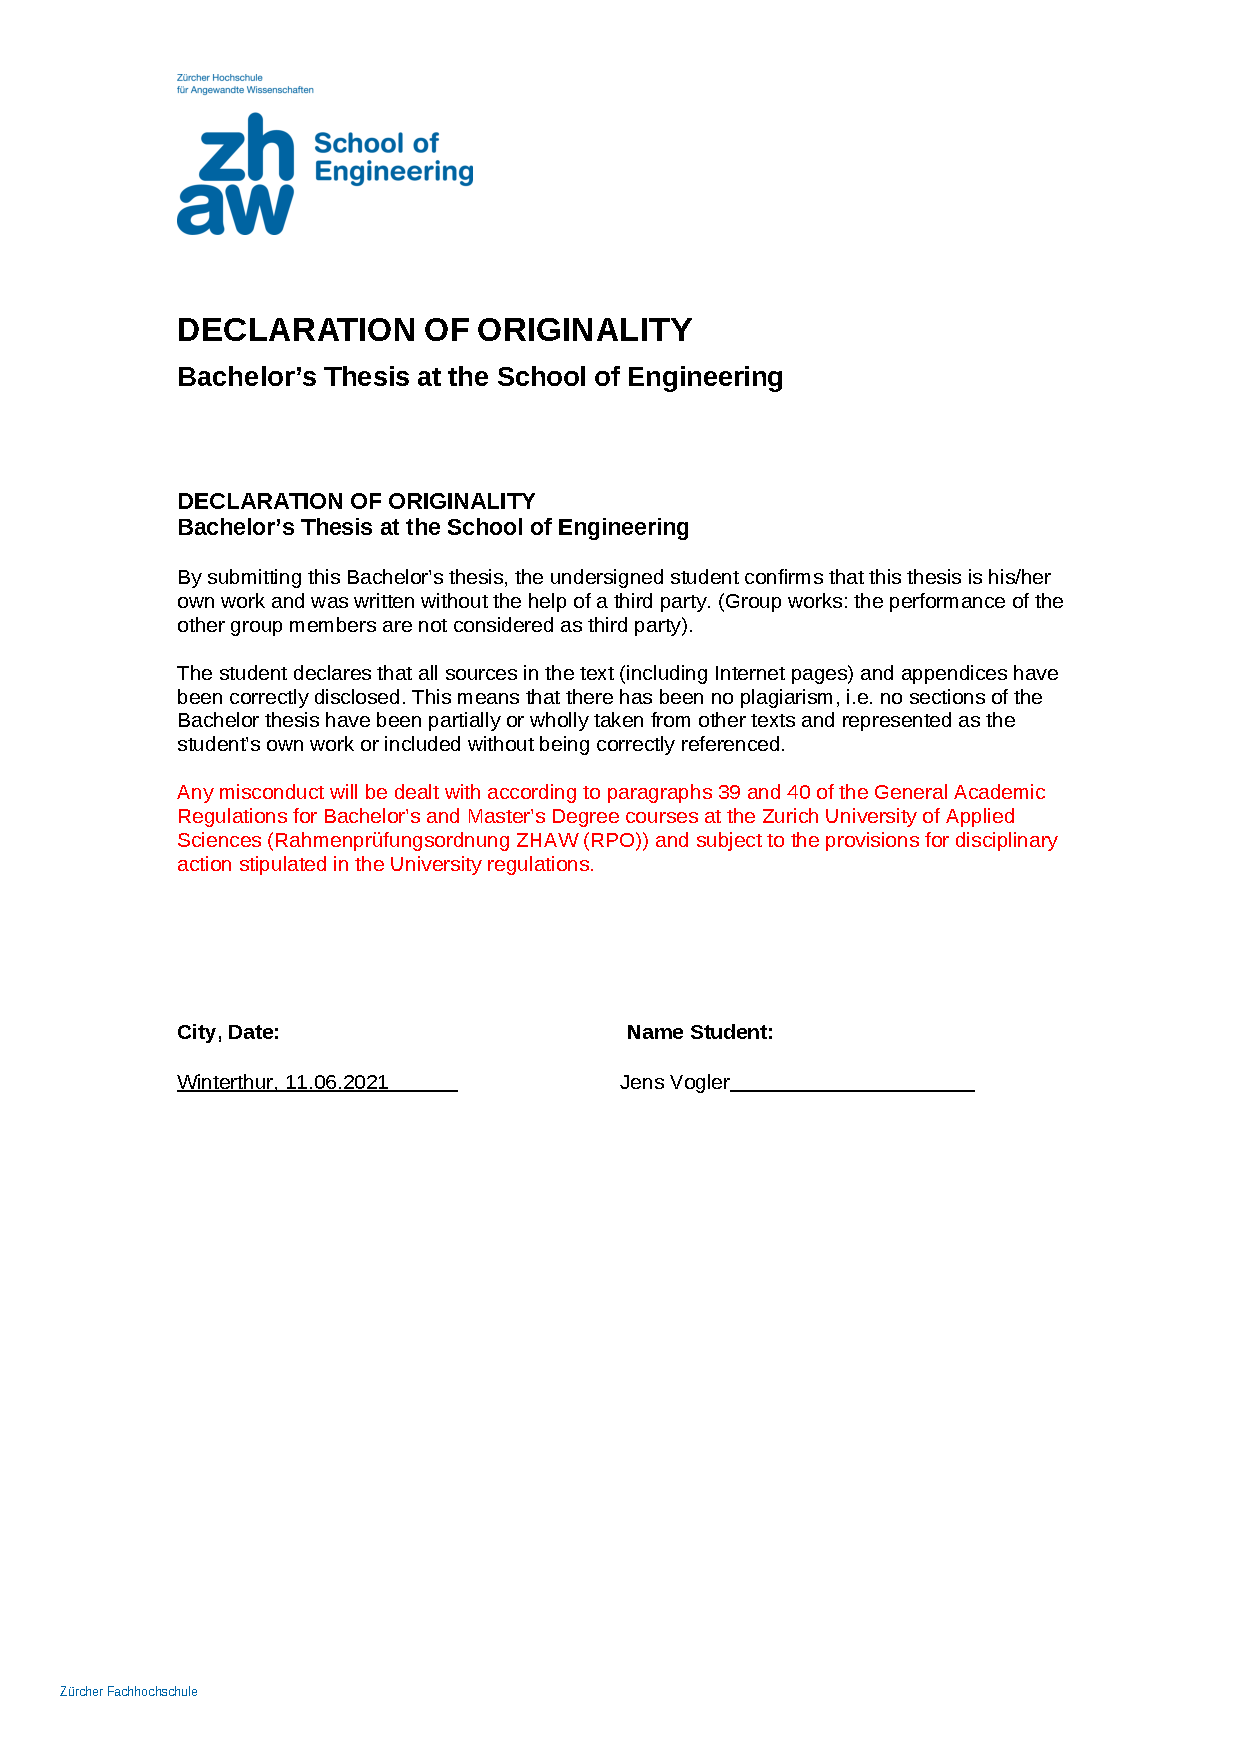
\includepdf[pages=-]{../Attachments/Erklaerung_BA_digital-_EN.pdf}


%** environments.tex: Predefined Environments
%****************************************************************************
%** Copyright 2002 by Lukas Ruf, ruf@topsy.net
%** Information is provided under the terms of the
%** GNU Free Documentation License http://www.gnu.org/copyleft/fdl.html
%** Fairness: Cite the source of information, visit http://www.topsy.net
%****************************************************************************

\newenvironment{sourcecode}%
{\vspace{0.5 cm} \footnotesize \verbatim}%
{\endverbatim \normalsize \vspace{0.5 cm}}

\newenvironment{inputverb}[1]%
{\vspace{0.5 cm} \footnotesize \verbatiminput{#1}}%
{\normalsize \vspace{0.5 cm}}

\newenvironment{inputverb_nospace}[1]%
{\footnotesize \verbatiminput{#1}}%
{\normalsize}


%**Documentation****************

%** Zusammenfassung.tex
\clearpage
\null
\vfil % or it might be \null
\begin{center}\textbf{Abstract}\end{center}

%** Vorwort.tex
\thispagestyle{empty}
\clearpage
\null
\vfil % or it might be \null
\begin{center}\textbf{Foreword}\end{center}

%** Table of Contents
\tableofcontents

%** Einleitung.tex: 
% - Nennt bestehende Arbeiten/Literatur zum Thema
% - Stand der Technik: Bisherige Lösungen des Problems und deren Grenzen
% - (Nennt kurz den Industriepartner und/oder weitere Kooperationspartner und dessen/deren Interesse am Thema Fragestellung)
% - Formuliert das Ziel der Arbeit
% - Verweist auf die offizielle Aufgabenstellung des/der Dozierenden im Anhang
% - (Pflichtenheft, Spezifikation)
% - Übersicht über die Arbeit: stellt die folgenden Teile der Arbeit kurz vor
% - (Angaben zum Zielpublikum: nennt das für die Arbeit vorausgesetzte Wissen)
% - (Terminologie: Definiert die in der Arbeit verwendeten Begriffe)
\chapter{\label{introduction}Introduction}
\thispagestyle{fancy}



%** TheoretischeGrundlagen.tex:
\chapter{\label{theory}Theory}
\thispagestyle{fancy}



%** Vorgehen.tex:
% - Beschreibt die Grundüberlegungen der realisierten Lösung (Konstruktion/Entwurf) und die Realisierung als Simulation, als Prototyp oder als Software-Komponente etc.
% - (Definiert Messgrössen, beschreibt Mess- oder Versuchsaufbau, beschreibt und dokumentiert Durchführung der Messungen/Versuche)
% - (Experimente)
% - (Lösungsweg)
% - (Modell)
% - (Eingesetzte Software)
% - (Tests und Validierung)
\chapter{\label{methods}Methods}
\thispagestyle{fancy}



%** Resultate.tex:
% - Zusammenfassung der Resultate
\chapter{\label{results}Results}
\thispagestyle{fancy}



%** DiskussionAusblick.tex:
% - Bespricht die erzielten Ergebnisse bezüglich ihrer Erwartbarkeit, Aussagekraft und Relevanz
% - Interpretation und Validierung der Resultate
% - Rückblick auf Aufgabenstellung, erreicht bzw. nicht erreicht
% - Legt dar, wie an die Resultate (konkret vom Industriepartner oder weiteren Forschungsarbeiten; allgemein) angeschlossen werden kann; legt dar, welche Chancen die Resultate bieten.
\chapter{\label{discussion}Discussion}
\thispagestyle{fancy}



%** Verzeichnisse.tex:
\chapter{\label{references}References}
\thispagestyle{fancy}

\raggedright
\printbibliography[title={Bibiliogrpahy},heading=subbibnumbered]
% [title={Literaturverzeichnis},heading=subbibnumbered] würde nummerieren

\pagebreak
\printglossary

%** Table of Figures
\pagebreak
\listoffigures

%** Table of Figures
\pagebreak
\listoftables

\pagebreak
\printglossary[type=\acronymtype]

%** Anhang.tex:

\chapter{\label{appendix}Appendix}
\thispagestyle{fancy}

%** end the document environment
\end{document}
